\section{Ingredient}\label{sec:ingredient}

\subsection{View Ingredient List}\label{sec:ingredient_list}
\setcounter{stepcounter}{1}
\paragraph{\arabic{stepcounter}.} Inorder to access list of ingredient click on \textcolor{ForestGreen}{"Ingredients"} menu from the sidebar.
\begin{figure}[h!]
  	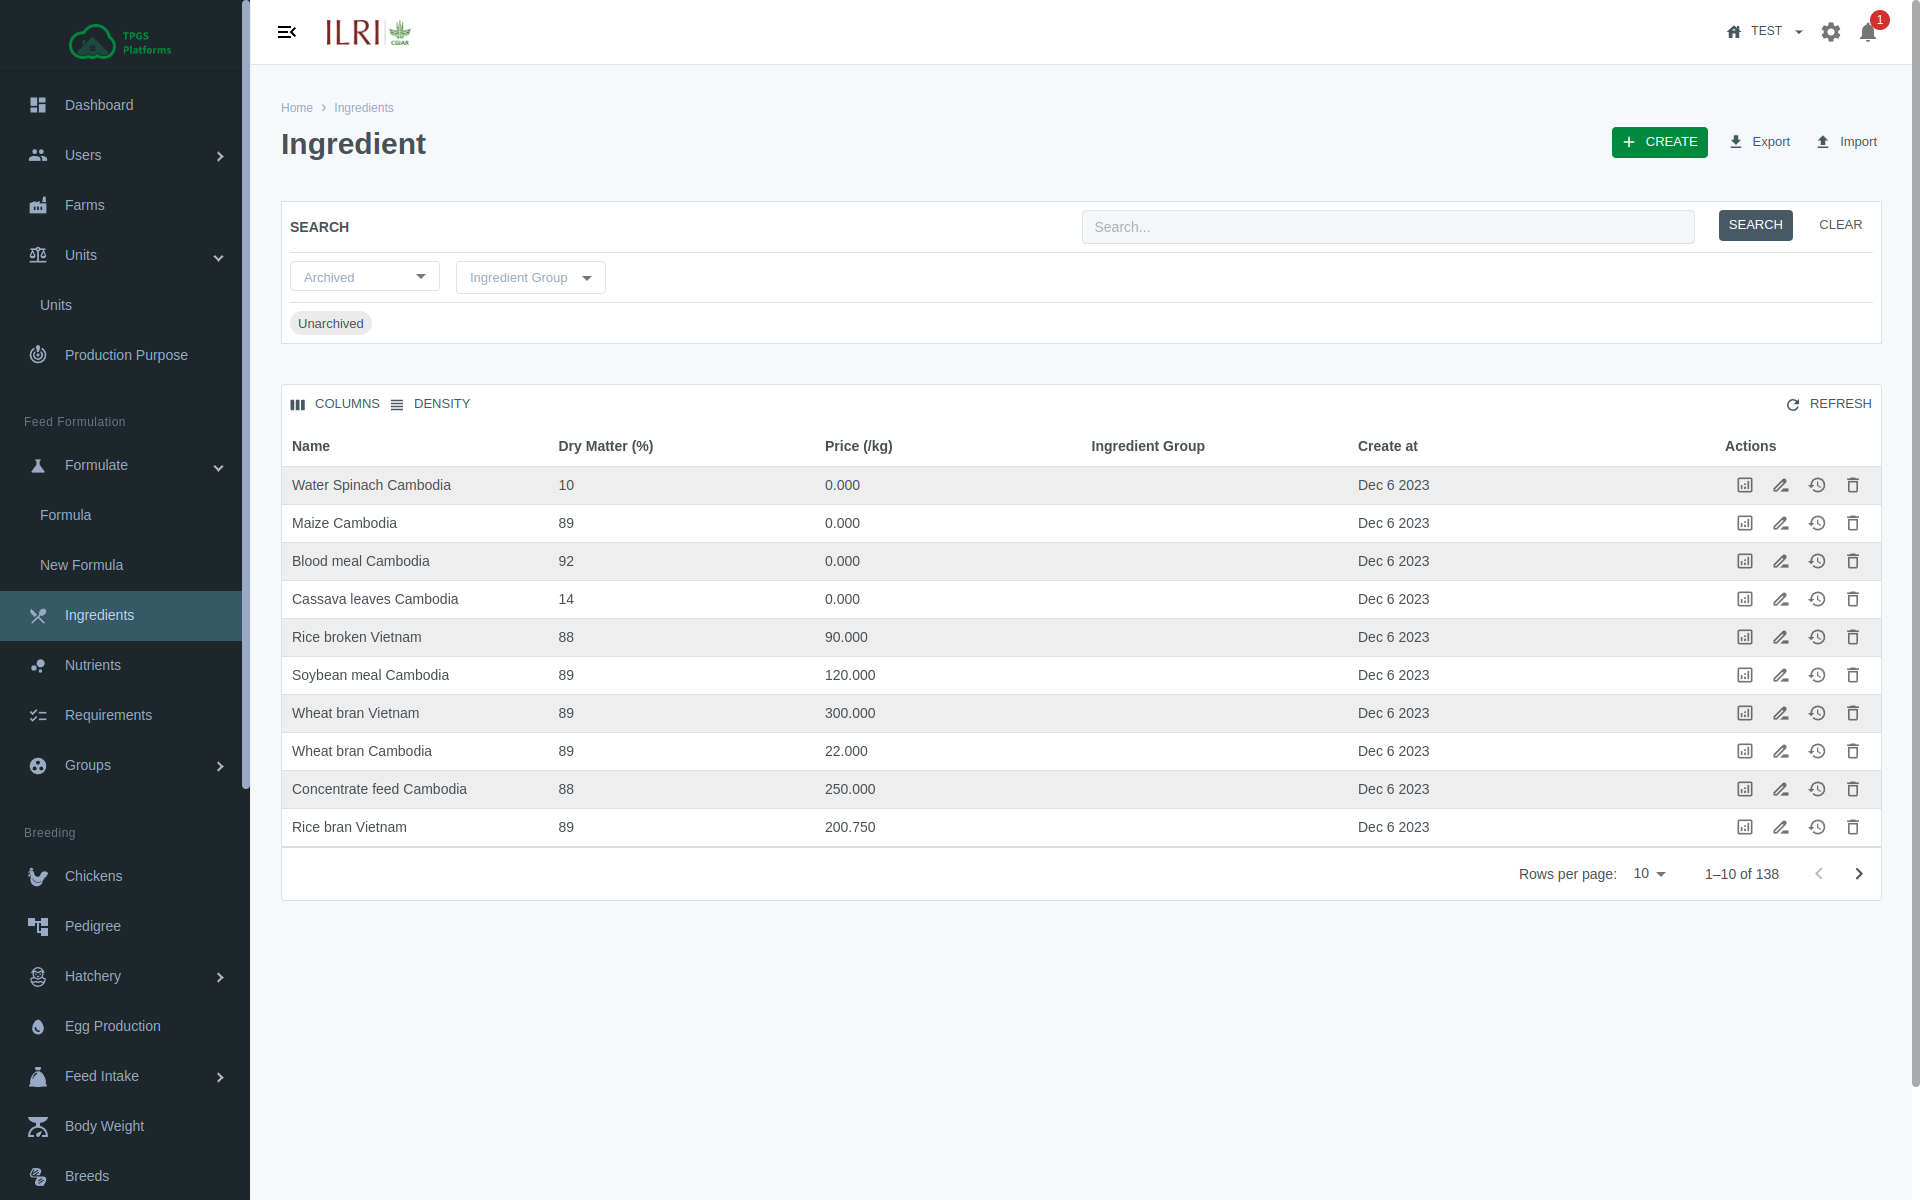
\includegraphics[width=15cm]{screenshots/ingredient_list_page.png}
  	\caption{Ingredients  List}
  	\label{fig:nutrient_list_page}
\end{figure}
\paragraph{\arabic{stepcounter}.} Filter the list of ingredients by using the \textcolor{ForestGreen}{"SEARCH"} card.

\subsection{Create new Nutrient }\label{sec:ingredient_create}
\setcounter{stepcounter}{1}
\paragraph{\arabic{stepcounter}.}To create new ingredient click on \textcolor{ForestGreen}{"Create"} from \hyperref[fig:ingredient_list_page]{Ingredients page \ref{fig:nutrient_list_page}}
\begin{figure}[h!]
  	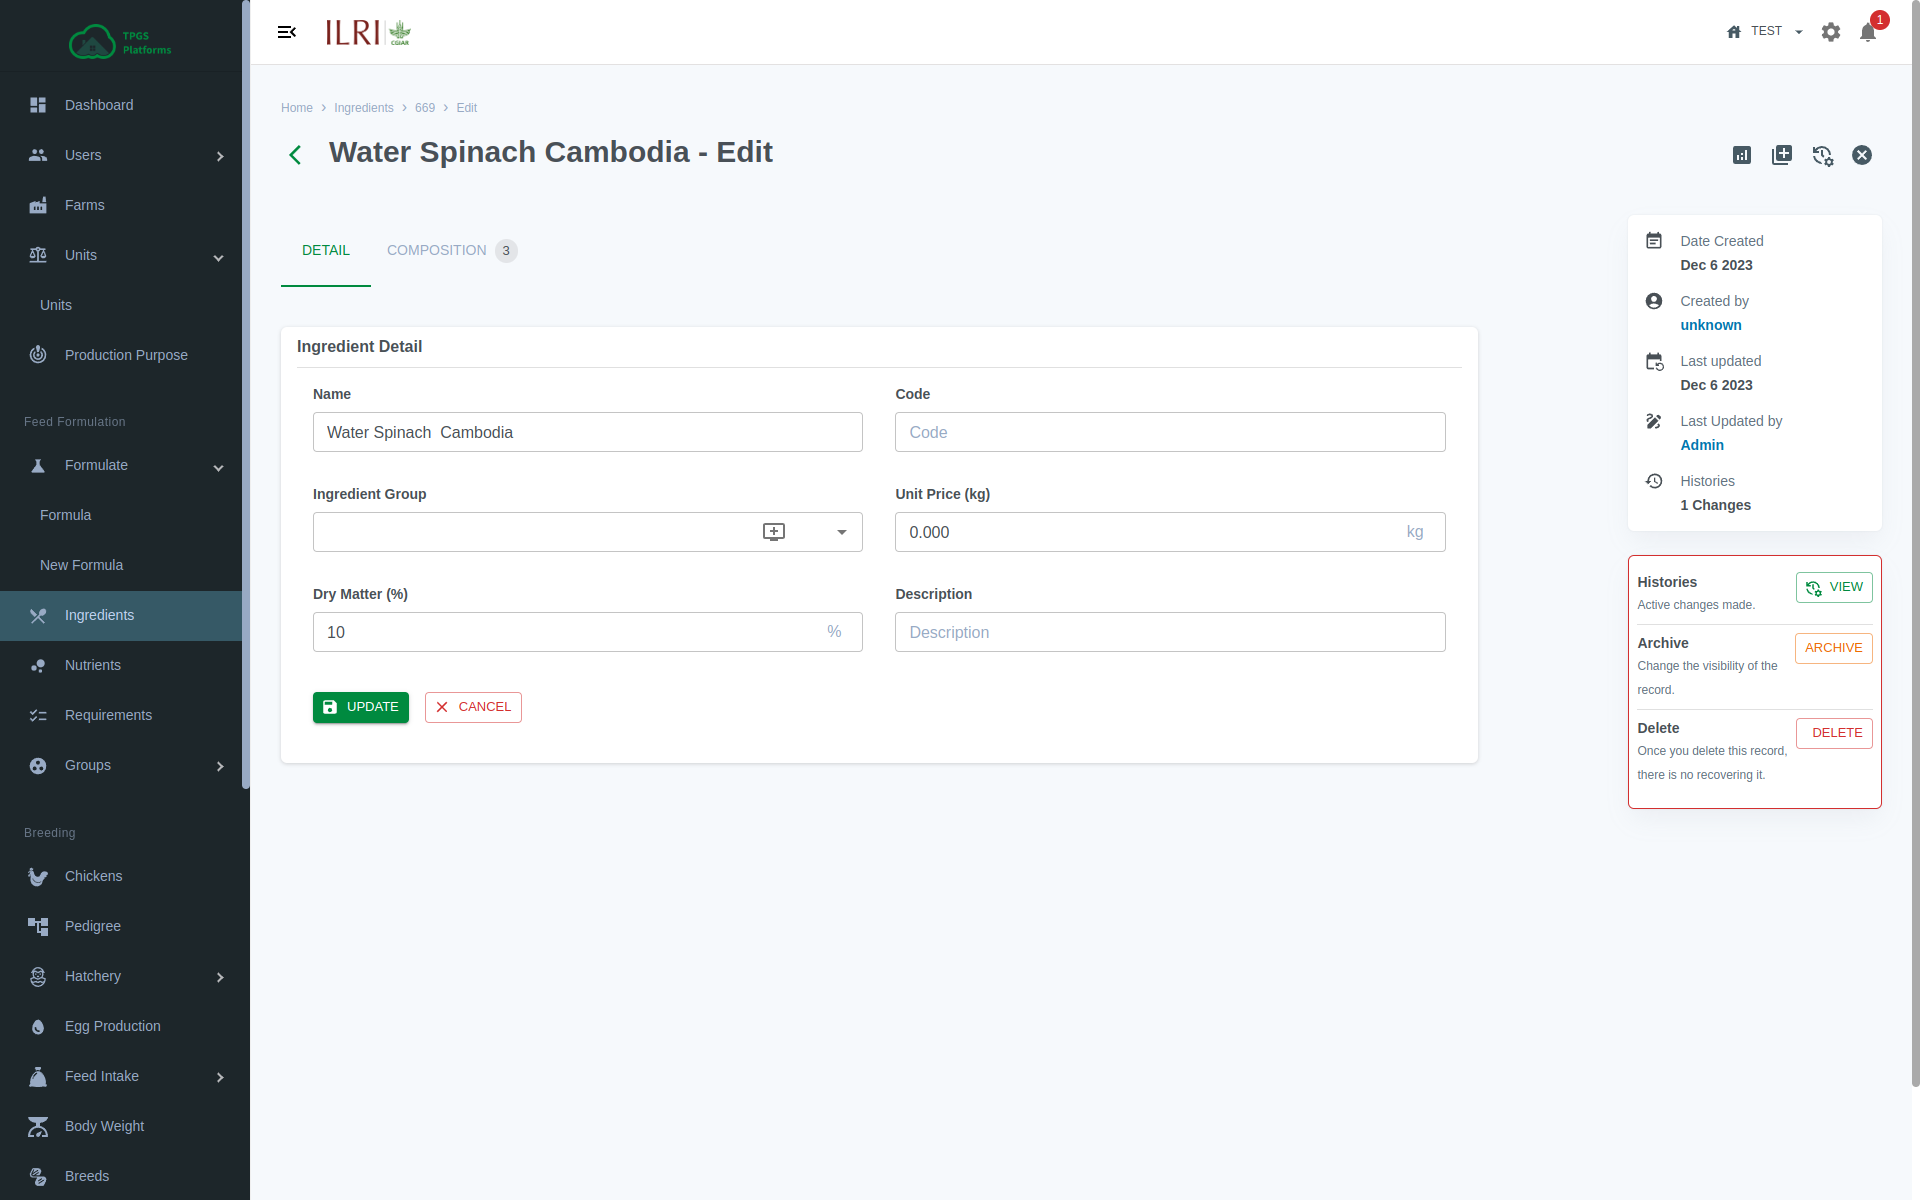
\includegraphics[width=15cm]{screenshots/ingredient_edit_page.png}
  	\caption{Create new Nutrient }
  	\label{fig:nutrient_create_page}
\end{figure}

\paragraph{\arabic{stepcounter}.} Input the necessary information about the ingredient and click on \textcolor{ForestGreen}{"CREATE"} button
\paragraph{\arabic{stepcounter}.} After the ingredient is created, a \textcolor{ForestGreen}{"COMPOSITION"} will appear at the top.
\paragraph{\arabic{stepcounter}.} Set ingredient's composition by clicking \textcolor{ForestGreen}{"Add New"} and choosing the type of nutrient.
\paragraph{\arabic{stepcounter}.} To set value to nutrient double click on value column to corsponding row, the value will be automatically saved once you are done editing.